\href{https://www.thedrum.com/about-us}{The Drum} is a market awareness website and \href{https://www.thedrum.com/news/2022/08/01/web3-the-numbers-key-metaverse-crypto-and-nft-stats-every-marketer-should-know}{compiled} the following statistics, which have been linked back to their source and annotated for our needs. 
\textit{\begin{itemize}
\item 89.4 million Americans are expected to use virtual reality (VR) in 2022, \href{https://www.insiderintelligence.com/content/us-augmented-virtual-reality-users-forecast-2022}{according to insiderintelligence}. That number, according to the same source, is expected to climb to 110.3 million in 2025. As a counter to this only around 16M VR headsets were sold in 2022
\item 51\% of gen Z and 48\% of millennials envision doing some of their work in the metaverse in the next two years, according to Microsoft’s Work Trend Index 2022.
\item 38\% of respondents said they would “try extreme sports like skydiving, bungee jumping, or paragliding” in the metaverse according to a recent Statista survey called ‘What things would you do in the metaverse but never in real life?’ Unsettlingly, 18\% of respondents said they would “conduct unethical experiments on virtual humans”
\item 87\% of Americans between the ages of 13-56 would be interested in engaging with a virtual experience in the metaverse “that is built around a celebrity they love,” according to new research from UTA and Vox Media
\item \$678bn is forecasted to be the total market valuation of the metaverse by 2030, per Grand View Research. According to the report, that market value was just shy of \item \$39bn in 2021, giving it a predicted compounded annual growth rate over a 10-year period of around 39%
\item 46\% of all people across age groups say that the ability to visualize a virtual product in an IRL context – “such as seeing a digital painting in their home using augmented reality (AR) glasses” – is the primary factor that would motivate them to make a purchase in the metaverse, per a Productsup survey
\item 24\% of US adult internet users say “that lower-priced VR headsets were a very important factor when deciding whether to try using the metaverse,” per a recent Statista survey. On the other hand, 54\% say that their workplace using the metaverse would “not [be] important at all” in their decision to give the metaverse a try
\item 15\% of gen Zs’ “fun budget” is spent in the metaverse, per a report from Razorfish and Vice Media Group. In five years that number is projected to climb to 20\%
\item Nearly 77\% believe that the metaverse “can cause serious harm to modern society,” per a recent survey from customer service platform Tidio. The survey, which received feedback from 1,000 participants, identified three major causes of anxiety related to the metaverse and its potentially negative social impacts: “addiction to a simulated reality” was the number one concern, followed by “privacy issues” and “mental health issues,” which were tied for second
\item By 2026, about 2 billion people worldwide “will spend at least one hour a day in the metaverse to work, shop, attend school, socialize or consume entertainment,” per McCann Worldgroup. By that same year, the total value of the virtual goods market in the metaverse could be as high as \$200bn
\item NFTs
Over \$37bn has been spent in NFT marketplaces as of May 2022, per data from Chainalysis. At their current rate, this year’s NFT sales could potentially surpass last year’s, which had a total valuation of around \$40bn, according to the data
\item \$91.8m was the sale price of ‘The Merge,’ the most valuable NFT to date. Created by the artist Pak, it sold for its record-breaking value in December 2021
\item 64\% of sports fans are open to the idea of learning more about NFTs and would consider purchasing one in the future, according to the National Research Group. The report also found that 46\% of sports fans “would be more likely to attend live sporting events if they were rewarded with a commemorative NFT – for example, if their ticket turned into a digital collectible after the game”
\item Only 9\% of people aged 16-44 own a NFT, and less than half (44\%) have purchased or invested in crypto, per a new survey from agency SCS. On the other hand, among the survey’s 600 respondents, 64\% were “aware” of the metaverse, and 65\% of that subgroup say they are “interested in exploring it further for everything from traveling to new places and playing games to making money and shopping”
\end{itemize}}
Polling company IPSOS \href{https://www.ipsos.com/en/global-advisor-metaverse-extended-reality-may-2022}{have conducted} a global survey for the World Economic Forum. Some highlights are:
\begin{itemize}
\item ``Excitement about extended reality is significantly higher in emerging countries than it is in most high-income countries. In China, India, Peru, Saudi Arabia, and Colombia, more than two-thirds say they have positive feelings about the possibility of engaging with it.''
\item ``Familiarity and favorability toward the new technologies are also significantly higher among younger adults, those with a higher level of education, and men than they are among older adults, those without a college-level education, and women.''
\end{itemize}

Excitingly for our exploration of the topic it can be seen in Figure \ref{fig:applications} that education within metaverse spaces is the most anticipated application, and we have seen that the emerging globals markets are the most optimistic about the technology overall. This is highly suggestive of an opportunity.

\begin{figure*}[ht]\centering % Using 
	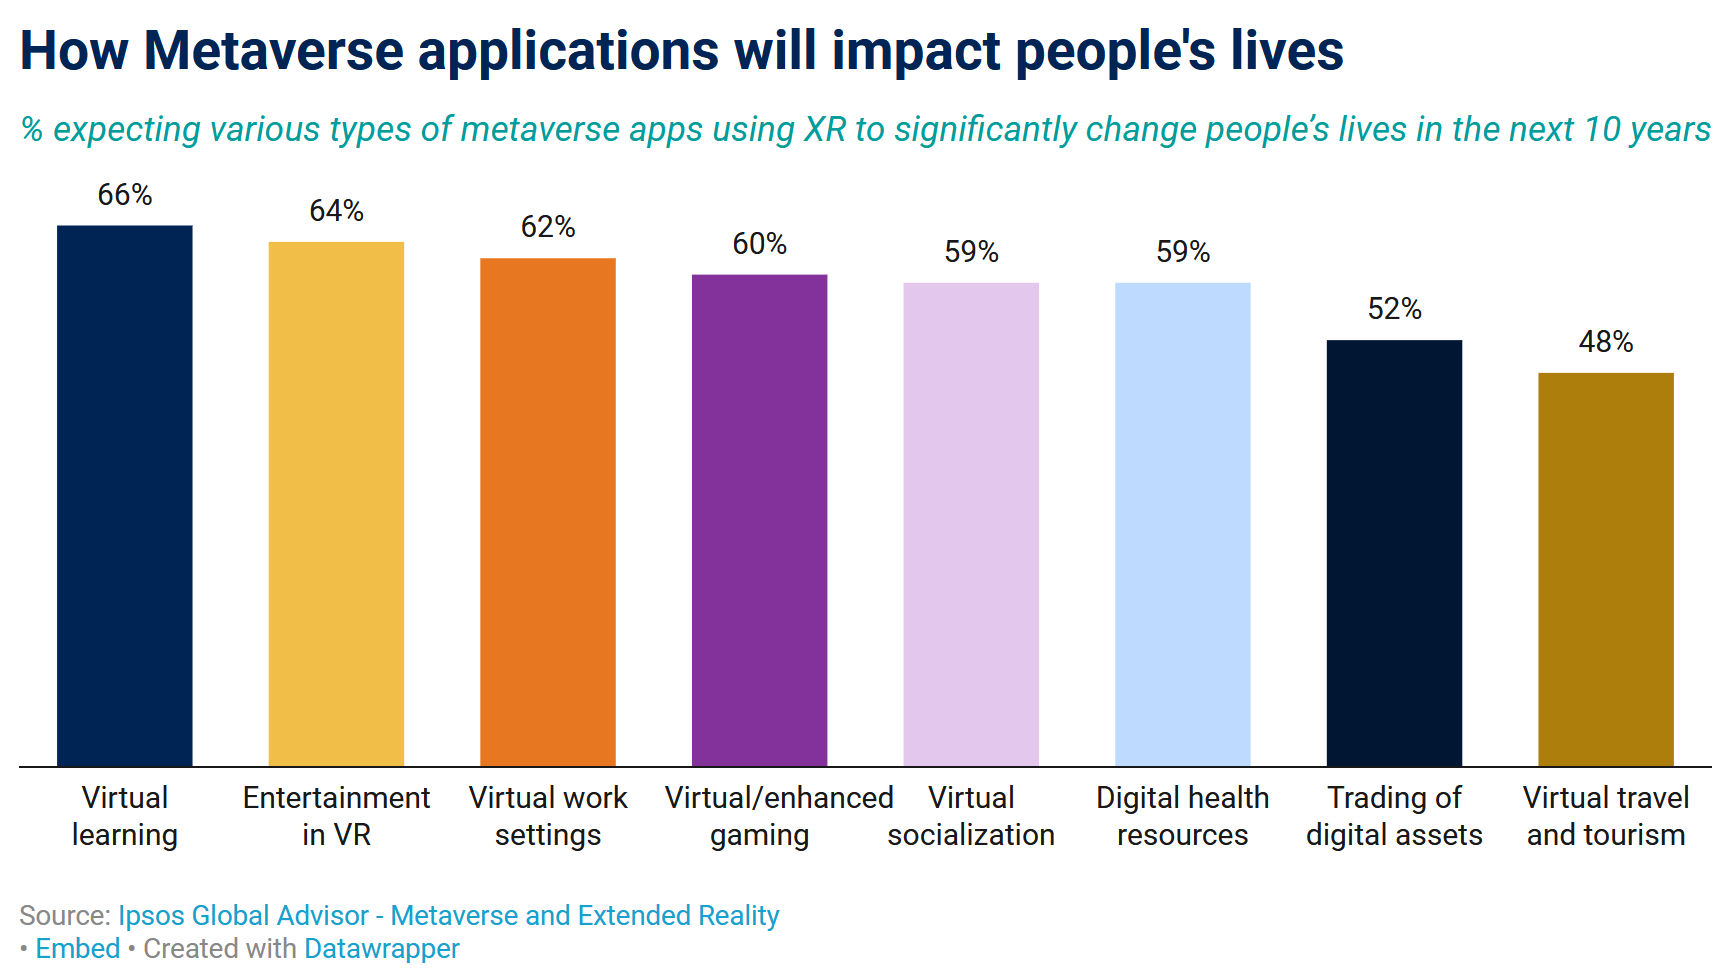
\includegraphics[width=\linewidth]{applications}
	\caption{\href{https://www.ipsos.com/en/global-advisor-metaverse-extended-reality-may-2022}{IPSOS poll predicted applications}}
	\label{fig:applications}
\end{figure*}

